\documentclass[a4paper,11pt,parskip=half,headings=small,DIV=11,notitlepage,abstract=on]{scrartcl}
% This file contains configuration shared between main file and figures

\usepackage{pifont}
\usepackage{xspace}
\DeclareUnicodeCharacter{2460}{\ding{172}\xspace}
\DeclareUnicodeCharacter{2461}{\ding{173}\xspace}

\usepackage{tikz}

\definecolor{HB9UFblue}{RGB}{0,61,165}
\definecolor{HB9UFred}{HTML}{ED135A}

\newcommand{\Ohm}{$\Omega$\xspace}


\newcommand{\uline}[1]{%
  \tikz[baseline=(todotted.base)]{
      \node[inner sep=1pt,outer sep=0pt] (todotted) {#1};
      \draw[color=HB9UFblue,thick] (todotted.south west) -- (todotted.south east);
  }%
}%
                           
\newcommand{\udash}[1]{%
  \tikz[baseline=(todotted.base)]{
      \node[inner sep=1pt,outer sep=0pt] (todotted) {#1};
      \draw[dashed,color=HB9UFred,thick] (todotted.south west) -- (todotted.south east);
  }%
}%

\usepackage{scrlayer-scrpage}
\usepackage{graphicx}
\usepackage{amsmath}
\usepackage[pdfauthor={},pdftitle={},pdfstartview=FitH,pdfborder={0 0 0}]{hyperref}
\usepackage[utf8]{inputenc}
\usepackage{textcomp}
\renewcommand{\thesection}{\Alph{section}}
\renewcommand*{\theenumi}{\thesection.\arabic{enumi}}

\usepackage{ngerman}
\ifoot{\texttt{}}
\ofoot{\texttt{}}

%\addtolength{\textheight}{10mm}
\title{Posten B\\Transmissionsmessungen an Filtern}
\author{}
\date{}
\pagestyle{empty}
\renewcommand*{\titlepagestyle}{empty}
\sloppy

\begin{document}
\maketitle
\vspace{-2cm}

An diesem Posten bestimmst du die Einfügedämpfung verschiedener Filter. Dabei
geht es stets darum, wieviel Leistung bei eingesetztem Prüfling zu Port ②
gelangt, verglichen mit der Leistung in Port ②, wenn der Prüfling nicht
eingesetzt ist:

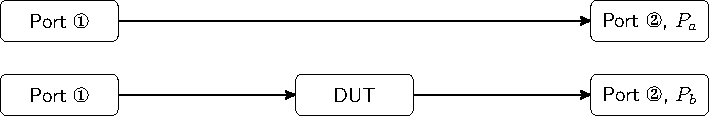
\includegraphics[width=\textwidth]{../skript/figures/dut_insertionloss/dut_insertionloss.pdf}

Dieses Verhältnis zwischen $P_a$ und $P_b$ wird in Dezibel (dB) angegeben. Eine Einfügedämpfung von 3~dB
bedeutet also, dass bei eingesetztem Prüfling nur noch die halbe Leistung zu
Port ② gelangt. Dabei spielt es keine Rolle, ob diese Einbusse aufgrund von
Reflexion am Eingang des Filters entsteht, oder durch Dissipation
(``verheizen'') im Filter -- in beiden Fällen ist das Resultat der Transmissionsmessung
3~dB, wobei man die zwei Fälle mit einer Reflexionsmessung natürlich unterscheiden
könnte. Der NanoVNA zeigt diese Einfügedämpfung, wie die meisten anderen
Geräte auch, eigentlich als Gewinn an. Im beschriebenen Beispiel wird deshalb
ein Resultat von -3~dB angezeigt.

Die folgende Illustration zeigt Beschaltung und Messresultat eines koaxialen
$\lambda/4$-Stubfilters. (Die ausgezogene Linie zeigt einen Stub mit
kurzgeschlossenem, die gestrichelte Linie einen mit offenen Ende.)

\vspace{5mm}
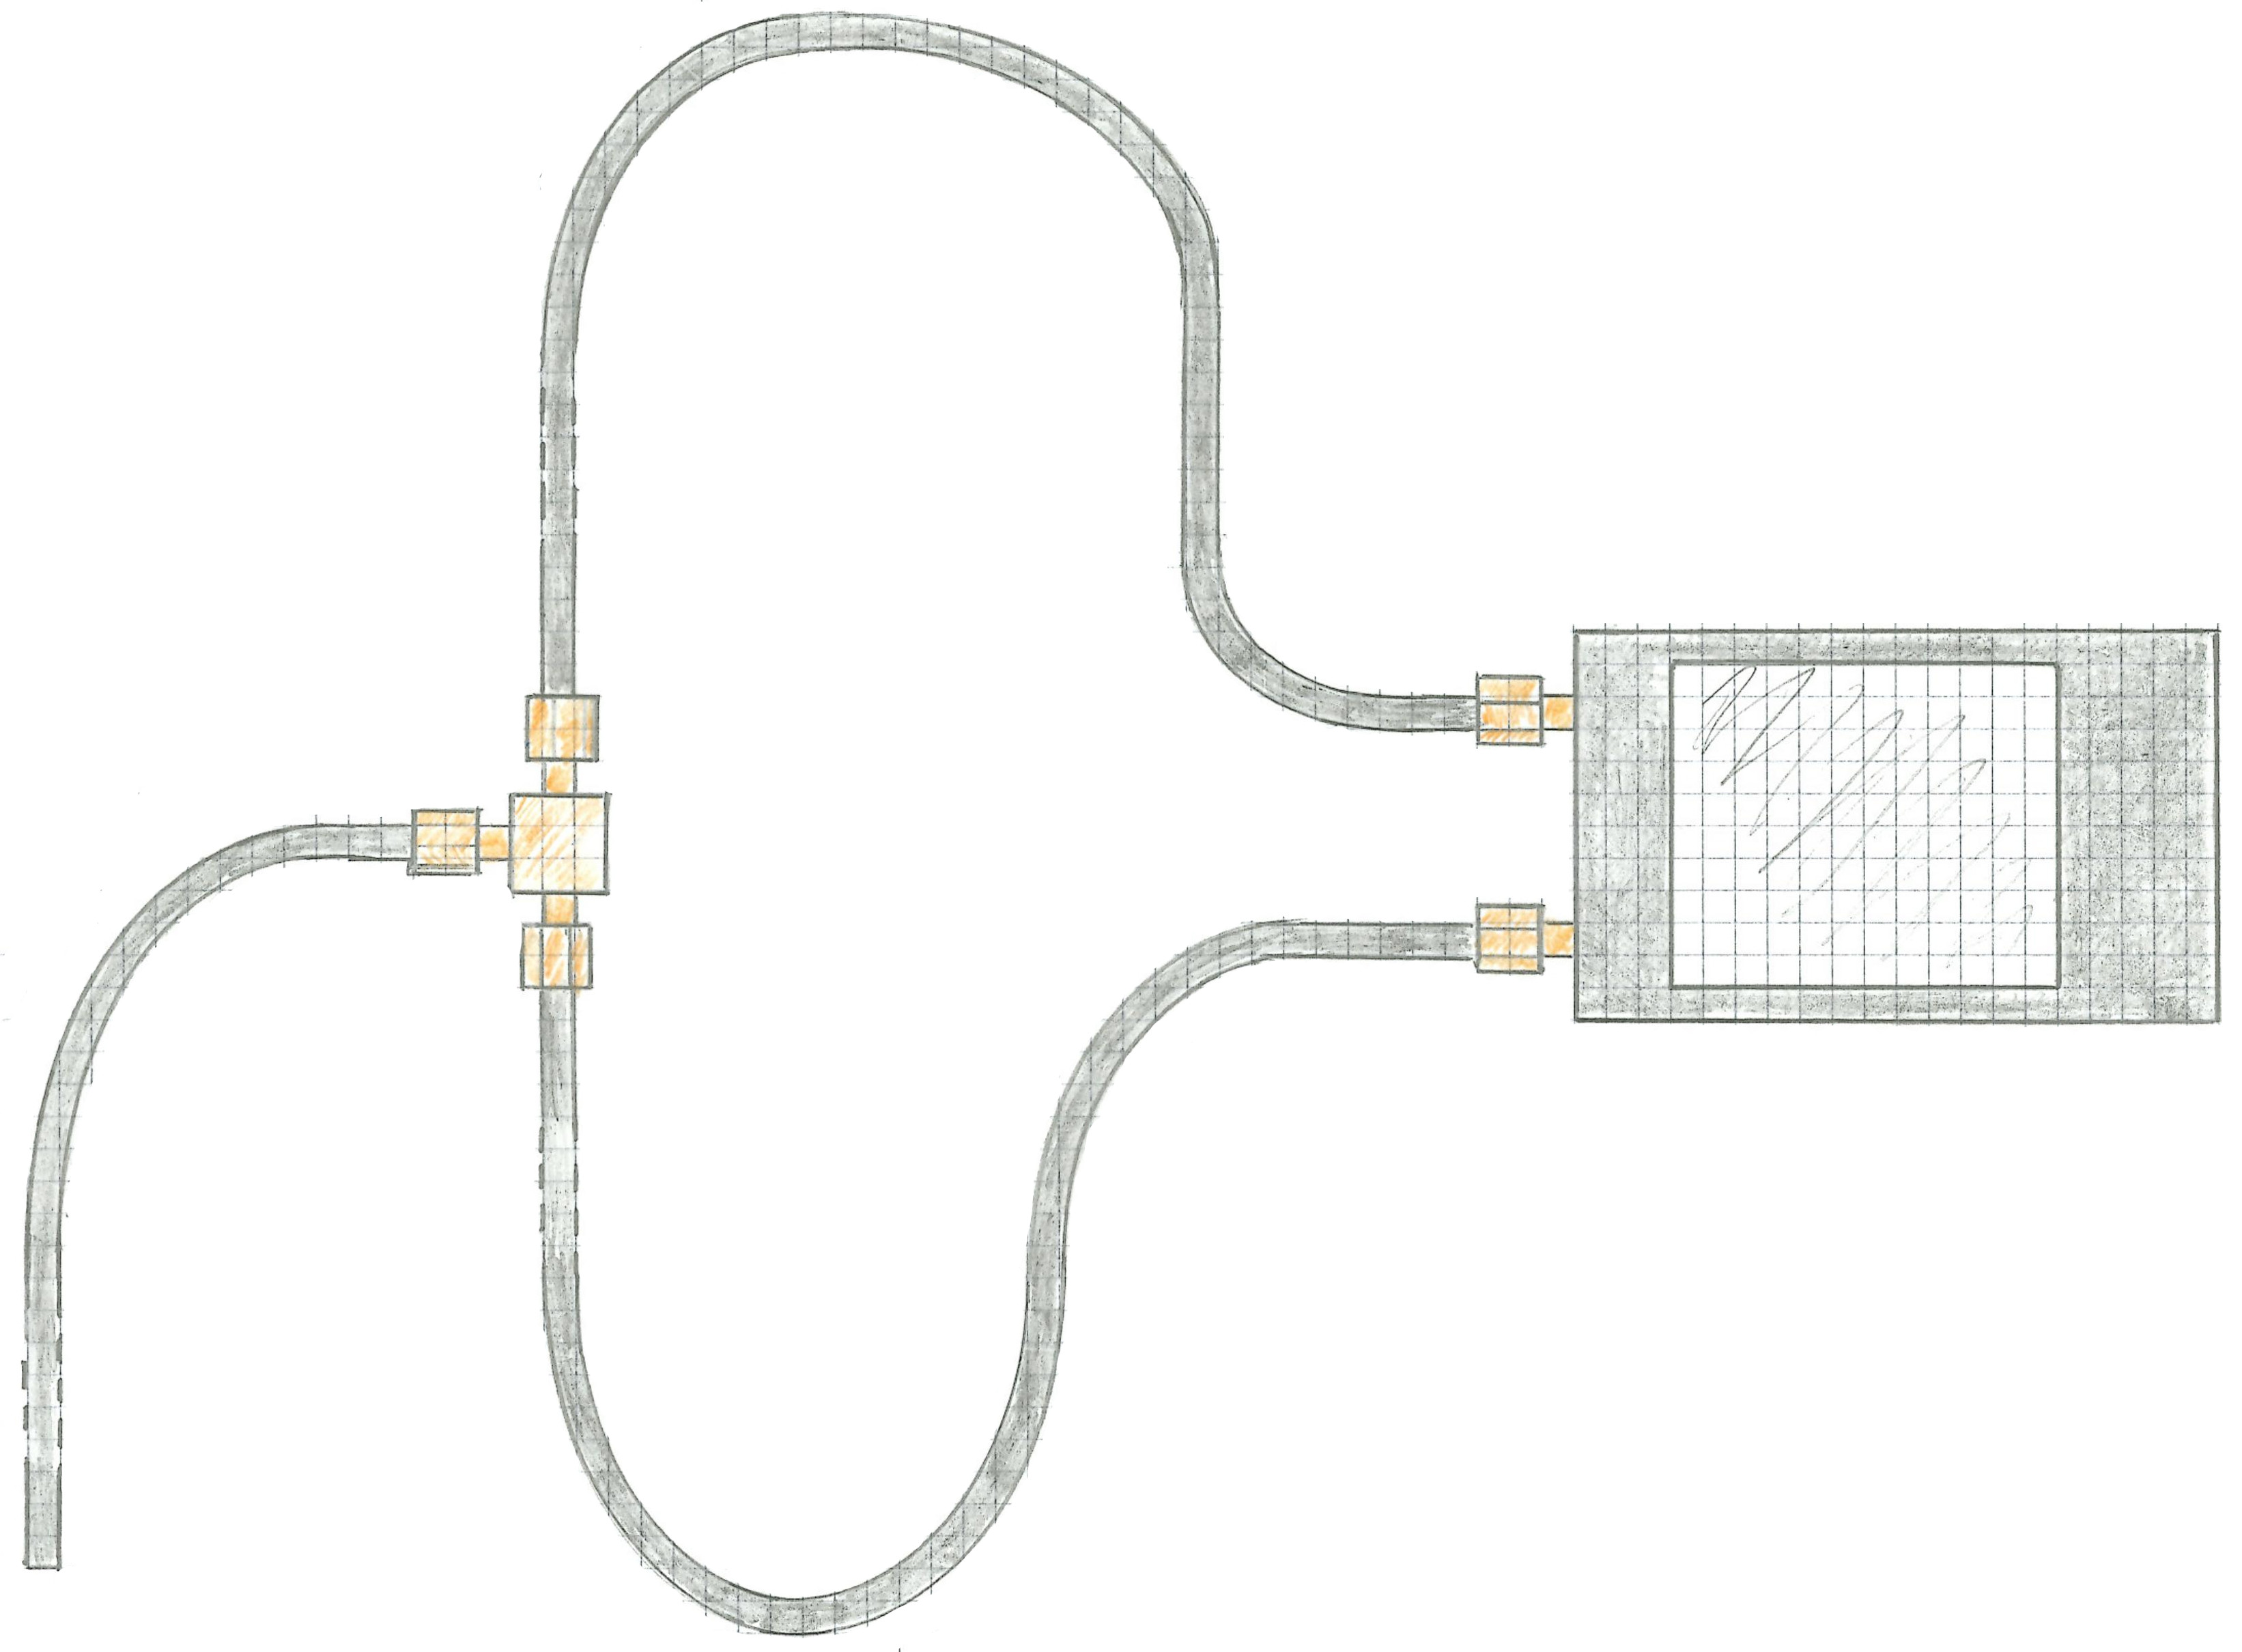
\includegraphics[height=3.6cm]{../skript/figures/illustration_stub.jpg}\hfill
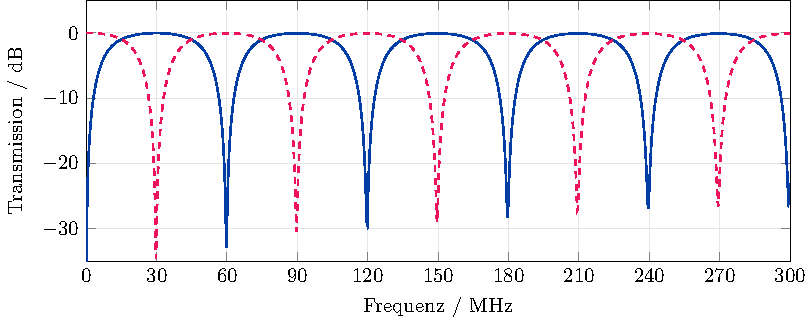
\includegraphics[height=3.6cm]{../skript/figures/stub/stub.pdf}

Es stehen verschiedene Filter und Dämpfungsglieder zum Aussmessen bereit: Hoch- und
Tiefpassfilter aus LC-Komponenten, $\lambda/4$-Stub, Schwingquarz, Kavität, SAW-Filter,
Duplexer, ... Lass dich von den Instruktoren anleiten, um diese Filter mit dem
Trace-Format ``LogMag'' auszumessen.

\end{document}
